\chapter{Statistical Inference} 
\chaptermark{Inference}
\label{sec:inference}

The idea of extrapolating knowledge from a \emph{sample} to a population is known as \emph{statistical inference}.
It encompasses the ideas of \emph{parameter estimation}, \emph{confidence intervals}, and \emph{hypothesis testing}.
We will assume the reader is familiar with these, but recall some required terminology.
The QC and SPC terminology are not always consistent with statisticians' terminology. When new names are given to old ideas, we will emphasize this in the text.

\begin{description}
\item [Null/Alternative Hypothesis] Some statement about the world we wish to test with data. The frequentist argument follows a Popperian philosophy\footnote{Following Karl Popper's philosophy of science, we can never know that something is true, we can only know when it is not true. Popper philosophy was motivated by the fact that no one suspected Isaac Newton's mechanics to be wrong, until relativity theory was proposed by Einstein.}: to show the alternative hypothesis is true, we will show that the null hypothesis is not true. 
In the context of quality control, the null hypothesis will be the process is \emph{in statistical control}, while the alternative will be that it is \emph{out of control}.\marginnote{In Control}
Other terms for the alternative hypothesis are the \emph{research hypothesis}, or simply the \emph{signal}.
\item [Statistical Test] The procedure of inferring from data on the truthfulness of the alternative hypothesis.
\item [Assumptions] As the name suggests, these are assumptions. We stress that unlike hypothesis, assumptions are not being tested in a statistical test. 
\item [Test Statistic] The function of the data to be computed for the purpose of inference. As such, it is a random variable. 
May also be though of as a \emph{signal detector}.
\item [Null/Alternative Distribution] The distribution of the test statistic under the null/alternative hypothesis.
\item [Type I/II error] See Figure~\ref{fig:confusion_table}.
\item [False/True Positive/Negative] See Figure~\ref{fig:confusion_table}.
\item [Rejection Region] The collection of event that will lead us to reject the null hypothesis, and believe in the alternative hypothesis.
\item [p-value] A.k.a. \emph{observed significance}. The null probability of the observed (or ``more extreme'') event.
\item [Significance Level] A.k.a. $\alpha$. The probability of a false positive.
\item [Power] The probability of a true positive.
\item [i.i.d.] ``Independent and identically distributed'' (i.i.d.) is an assumption made on the sampling distribution, meaning that samples are statistically independent, and all originating from the same distribution.

\end{description}

\begin{figure}
\centering
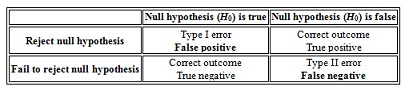
\includegraphics[width=0.8\linewidth]{art/Beware-of-False-Positives-Chart-1}
\caption[Confusion Table]{Type I/II error confusion table. \newline \url{https://infocus.emc.com/william_schmarzo/beware-of-false-positives/}}
\label{fig:confusion_table}
\end{figure}


The following sections of this chapter present particular statistical inference methods we will be using in the following chapters.


\begin{think}
Can you design a test with type I error larger its power?
Would you ever want such a test?
Think about it using the analogy to statistical tests and criminal courts. 
\end{think}


\section{Goodness of Fit (GOF)}
\sectionmark{GOF}
\label{sec:gof}

Goodness of fit (GOF) deals with the inference on the sampling distribution, a.k.a., the generative process.
It can be approached via rigorous hypothesis testing, or by visualizations.




\subsection{QQplot and QQnorm}
\label{sec:qqplot}

The fundamental idea of the \emph{quantile-quantile plot} (QQplot) is to compare the empirical quantiles in the sample, to the theoretical quantiles implied by the assumed distribution. If the theory and observations agree, we conclude our assumptions are plausible. 
For the particular case of testing the normality of the data, the corresponding QQplot is known as a \emph{QQnorm plot}.

Figure~\ref{fig:qqnorm_normal} illustrates a QQnorm plot of normal distributed data, while Figure~\ref{fig:qqnorm_non_normal} is the same for non-normal data.


\begin{figure}[h]
\centering
\begin{minipage}{0.45\textwidth}
\centering
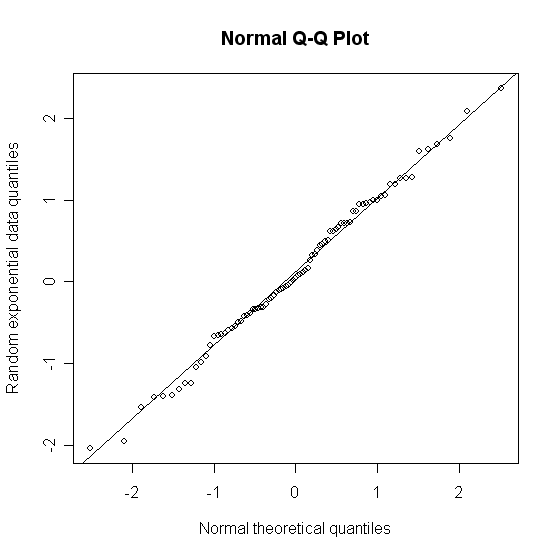
\includegraphics[height=0.3\textheight]{art/Qqnorm}
\caption[QQnorm- Gaussian]{A QQplot of Gaussian distributed data.}
\label{fig:qqnorm_normal}
\end{minipage}\hfill
\begin{minipage}{0.45\textwidth}
\centering
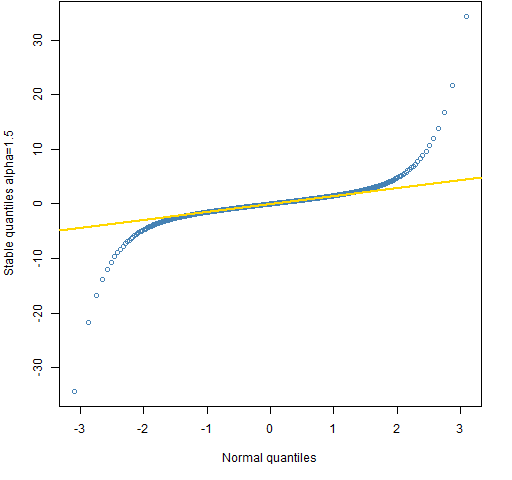
\includegraphics[height=0.3\textheight]{art/stab15qqnorm}
\caption[QQnorm- non Gaussian]{A QQnorm plot of non Gaussian distributed data.}
\label{fig:qqnorm_non_normal}
\end{minipage}
\end{figure}




\subsection{Chi-Square GOF Test}
The Chi-Square GOF test (not to be confused with the Chi-Square independence test), tests a hypothesis on the sampling distribution of discrete (attributes) data. 
Note that it is very general, since all continuous variables may be discretized, simply by binning.

\begin{definition}[Chi-Square GOF Test]
Assume an i.i.d. sample $x_1,\dots,x_n$. 
The Chi-Square GOF is a tests $H_0: \x_i \sim \dist$ versus $H_1: \x_i \not\sim \dist$.
$P$ is assumed to be discrete with $K$ categories and $p_k:= \dist(\x_i \in k)$.
The test statistic, $X^2$, is defined as
\begin{align}
	X^2:= \sum_{k=1}^{K}\frac{(obs_k-exp_k)^2}{exp_k}, 
\end{align}
where $obs_k:= \#\set{x_i \in k}$, and $exp_k:= p_k n$.
The approximate null distribution of $X^2$ is $\chi^2_{K-1}$.
\end{definition} 



\subsection{Kolmogorov–Smirnov GOF Test}
The Kolmogorov-Smirnof GOF test, tests a hypothesis on the sampling distribution of continuous (variable) data. 

\begin{definition}[Kolmogorov–Smirnov GOF Test]
Assume an i.i.d. sample $x_1,\dots,x_n$. 
The Chi-Square GOF is a tests $H_0: \x_i \sim \dist$ versus $H_1: \x_i \not\sim \dist$.
$P$ is assumed to be continuous.
The test statistic, $D$, is depicted in Figure~\ref{fig:ks_test}.
The null distribution of $D$ is the \emph{Kolmogorov distribution} obtained from tables.\marginnote{Kolmogorov Distribution}

\begin{figure}
\centering
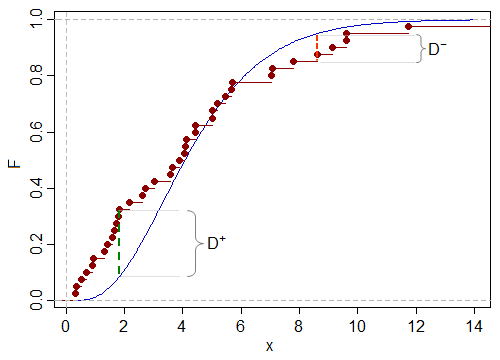
\includegraphics[height=0.3\textheight]{art/Kgn0O}
\caption[Kolmogorov-Smirnov Test]{Kolmogorov-Smirnov Test. The $D$ statistic is $D_+$ in the figure.}
\label{fig:ks_test}
\end{figure}

\end{definition} 






\begin{extra}[GOF tests]
There are endlessly many more GOF tests, such as Anderson-Darling, Jarque–Bera, Shapiro–Wilk, Kuiper's test, etc.
Wikipedia is a good place for further reading.
\end{extra}
